\documentclass[11pt]{report}
\usepackage[letterpaper, total={6.5in, 10in}]{geometry}
%\usepackage{fancyhdr}
%\pagestyle{fancy}
\usepackage{amsmath, amsthm, mathpazo, epic, eepic, color, array}
\usepackage{amssymb}
%\usepackage{graphicx}
\usepackage{cancel}
\usepackage{pgfplots}
\usepackage{multicol}
\pgfplotsset{compat=1.13}
\usepackage{etoolbox}
\makeatletter
\patchcmd{\chapter}{\if@openright\cleardoublepage\else\clearpage\fi}{}{}{}
\makeatother
\usepackage{hyperref}

\usepackage{enumerate}
\usepackage{enumitem}

\usepackage{tikz}
\usetikzlibrary{positioning,chains,fit,shapes,calc,arrows,patterns}
\usepackage{tkz-graph}
\usetikzlibrary{arrows, petri, topaths}
\usepackage{tkz-berge}
\usepackage[all]{xy}
\usepackage{textcomp}

\newboolean{colorprint}
\setboolean{colorprint}{true}
%\setboolean{colorprint}{false}

\ifthenelse{\boolean{colorprint}}{%
\newcommand{\colorone}{blue}
\newcommand{\colortwo}{red}
\newcommand{\coloronefill}{blue!15!white}
\newcommand{\colortwofill}{red!15!white}
\newcommand{\colormapone}{rgb=(.4,.4,1); rgb=(.8,.8,1)}
\newcommand{\colormaptwo}{rgb=(1,.4,.4); rgb=(1,.8,.8)}
\newcommand{\colormapplaneone}{rgb=(.7,.7,1); rgb=(.9,.9,1)}
\definecolor{colormaponebottom}{rgb}{.4,.4,1}
\definecolor{colormaponetop}{rgb}{.8,.8,1}
\definecolor{colormaptwobottom}{rgb}{1,.4,.4}
\definecolor{colormaptwotop}{rgb}{1,.8,.8}
}% ends color
{% not color
\newcommand{\colorone}{black}
\newcommand{\colortwo}{black!50!white}
\newcommand{\coloronefill}{black!15!white}
\newcommand{\colortwofill}{black!05!white}
\newcommand{\colormapone}{rgb=(.4,.4,.4); rgb=(.7,.7,.7)}
\newcommand{\colormaptwo}{rgb=(.6,.6,.6); rgb=(.9,.9,.9)}
\newcommand{\colormapplaneone}{rgb=(.8,.8,.8); rgb=(.95,.95,.95)}
\definecolor{colormaponebottom}{rgb}{.4,.4,.4}
\definecolor{colormaponetop}{rgb}{.7,.7,.7}
\definecolor{colormaptwobottom}{rgb}{.6,.6,.6}
\definecolor{colormaptwotop}{rgb}{.9,.9,.9}
}%

\newlength\tindent
\setlength{\tindent}{\parindent}
\setlength{\parindent}{0pt}
\renewcommand{\indent}{\hspace*{\tindent}}

\pgfplotsset{my style/.append style={axis x line=middle, axis y line=
middle, xlabel={$x$}, ylabel={$y$}, axis equal }}

\pgfplotsset{compat=1.13}

\usepackage[normalem]{ulem}

\begin{document}

{\bf Chapter 2: Derivatives}\\

%%%%%%%%%%%%%%%%%%%%%%Section 2.5%%%%%%%%%%%%%%%
{\bf Section 2.5 The Chain Rule}
\vskip .25 truein

All page numbers refer to original APEX text page numbers.\\
\\
\textbf{p. 97} \\
After Chain Rule box
We can think of this as taking the derivative of the outer function evaluated at the inner function times the derivative of the inner function. To help...Example 59.
\vskip .25 truecm

\textbf{pp. 98-99} \\
Sentence right before Generalized Power Rule box add bracketed text:\\
"Example 60....$f(x)=x^n$ [and $y=f(g(x))$], then..."
\vskip .25 truecm

\textbf{Generalized Power Rule}
change restriction on $n$ to any real number.
\vskip .25 truein 

For problem before Example 61 add step to show CR details:\\
$y' \displaystyle{= 20(3x^2 -5x +7 + \sin x)^{19} \cdot  \frac{d}{dx} (3x^2 -5x +7 + \sin x)}$
\vskip .5 truecm

Similarly in Example 61 insert additional steps in the solutions.\\ 
For \#1: insert $\cos (2x) \cdot \frac{d}{dx}(2x)=$\\
For \#2: insert $= \frac{1}{4x^3-2x^2} \cdot \frac{d}{dx} (4x^3-2x^2)$\\
For \#3: insert $=e^{x^2} \cdot \frac{d}{dx}(x^2)$
\vskip .25 truecm

Example 62 solution in last line of text insert bracketed word: "...Thus the equation of the ...is [approximately]"
\vskip .25 truecm

In line:  $\displaystyle{\frac{d}{dx}\left(\ln (\text{anything})\right) =...}$ use $\frac{d}{dx}$ instead of ' to indicate derivative.
\vskip .25 truecm

\textbf{p. 100} \\
In Example 63 insert additional steps in the solutions.\\ 
For \#1: insert $\displaystyle{= x^5 \cdot \frac{d}{dx}(\sin 2x^3) + \frac{d}{dx}(x^5) \cdot \sin 2x^3 = x^5 \cdot [\cos 2x^3 \cdot \frac{d}{dx}(2x^3)] + 5x^4 \cdot \sin 2x^3}$\\
\\
For \#2: insert $\displaystyle{= \frac{e^{-x^2} \cdot \frac{d}{dx}(5x^3) - 5x^3\frac{d}{dx}e^{-x^2}}{(e^{-x^2})^2} = \frac{e^{-x^2} \cdot 15x^2 - 5x^3 \cdot e^{-x^2} \cdot \frac{d}{dx}(-x^2)}{(e^{-x^2})^2}=... }$
\vskip .5 truecm

\textbf{pp. 101-102} \\

Example 64 in paragraph below $y'$: "The function is frankly...several \sout{simple} small steps and be..."
\vskip .25 truecm

Change Example 65 to\\
\\
$f(x) = \displaystyle{\frac{x\cos (x^{-2}) -\sin^2(e^{4x}) }{\ln x^2}}$\\
\vskip .25 truecm
Tim: I think this solution will fit in the solution will fit in the space allowed with only one line in the numerator. Let me know if it doesn't.
\vskip .25 truecm
{\tiny $= \displaystyle{\frac{(\ln x^2) [-x(\sin x^{-2})(-2x^{-3}) + 1\cdot (\cos (x^{-2})) -2 \sin e^{4x} \cos e^{4x} \cdot (4e^{4x})] - \frac{1}{x^2} (2x) \cdot [x\cos (x^{-2}) -\sin^2(e^{4x})]}{(\ln x^2)^2}}$}
\vskip .25 truecm
In paragraph below this derivative: "The reader is highly... \sout{(I.e., the Quotient... term, etc.)} This example..."
\vskip .5 truecm

\textbf{pp. 102-103} \\

Move example 66 through Theorem 20 to Calculus II somewhere - I think Ricard has this part.
\vskip .25 truecm

I changed my mind about the use of "cancel" on this p. 103. \\
In paragraph: "Here the "fractional"... terms \sout{cancel} divide out, leaving."\\
In paragraph: "It is important to realize that we are not \sout{canceling} dividing these terms..."
\vskip 1 truecm

\textbf{Exercises}\\

Cut $a^x$-type problems. This means \# 19, 20, 22-25, 36b ( I think I got that's all of them)
\vskip .5 truecm 

Add:\\
\textbf{After current \#11:}\\
$\displaystyle{p(x) = \left(x^2 - \frac{1}{x^2}\right)^6}$\\

\indent Answer: $\displaystyle{p'(x) = 12\left(x^2 - \frac{1}{x^2}\right)^5 \left(x + \frac{1}{x^3}\right)}$\vskip 1 truecm


\textbf{After current \#15:}\\
$g(x) = \tan^2 x - \tan (x^2)$\\

\indent Answer: $g'(x) = 2(\tan x \sec^2 x - x \sec^2 (x^2))$\\

$w(x) = \sec (e^{x^3})$\\

\indent Answer: $w'(x) = 3x^2 e^{x^3}(\sec e^{x^3})(\tan e^{x^3})$\\
\vskip 1 truecm


\textbf{After current \#21:}\\
$\displaystyle{r(x) = \frac{\sqrt {4x-3}}{x^2}}$\\

\indent Answer: $\displaystyle{r'(x) = \frac{-6(x-1)}{x^3 \sqrt {4x-3}}}$\\


$\displaystyle{f(x) = \frac {(3x^2 - 5)^4}{(2x^3-1)^2}}$\\

\indent Answer: $\displaystyle{f'(x) = \frac {12x(2x^3-1)(3x^2 - 5)^3(x^2+5x-2)}{(2x^3-1)^4}}$\\
$h(x)=[(2x+1)^{10} + 1]^{10}$\\

\indent Answer: $h'(x)=200(2x+1)^9[(2x+1){10}+1]^9$\\

$\displaystyle{f(t)=\left[\left(1+ \frac{1}{t}\right)^{-1} + 1\right]^{-1}}$\\

\indent Answer: $\displaystyle{\frac{-t^4}{(2t+1)(t+1)}}$\\

$F(x)=2x(2x+1)^2 (2x+3)^3$\\

\indent Answer: $F'(x)=2(2x+1)(2x+3)^2(24x^2+26x+3)$\\
\vskip 1 truecm

\textbf{After current \#28:}\\

$a(t) = 7t^3e^{\tan t^2}$

\indent Answer: $a'(t)=7t^2 e^{\tan (t^2)}(2t^2 \sec^2 (t^2) + 3)$\\

$y=\sqrt{\sin (\cos^2 x)}$\\

\indent Answer: $\displaystyle{y'=\frac{-\cos x \sin x \cos (\cos^2 x)}{\sqrt{\sin (\cos^2 x)}}}$\\


$k(x) = \cos(x\sin x^3)$\\

\indent Answer: $k'(x) = -\sin(x\sin x^3)(3x^3\cos x^3 + \sin x^3)$\\

\vskip .5 truecm

If $k(x) = f(g(x)$ with $f(2)=-4, g(2)=2, f'(2)=3, \text{and } g'(2)=5$. Find $k'(2)$.\\

Suppose $r(x)=f(g(h(x)))$, where $h(1) = 2, g(2)=3, h'(1)=3, g'(2)=5,$ and $f'(3)=6$. Find $r'(1)$.
\vskip .5 truecm

\indent Answer: $15$\\

If $f$ and $g$ are functions whose graphs are shown, evaluate the expressions.\\
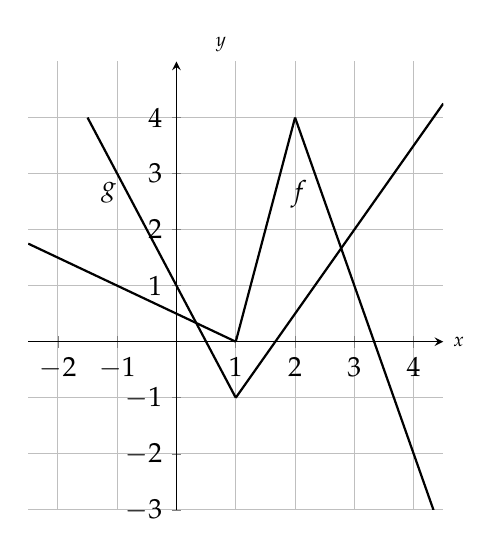
\begin{tikzpicture}
\begin{axis}[axis y line=middle,axis x line=middle, ymajorgrids=true, xmajorgrids=true, ymin=-3,ymax=5, xmin=-2.5,xmax=4.5, name=myplot, xscale=1/1.3, ytick={-3,-2,-1,0,1,2,3,4}]
\addplot [{\colorone}, domain=-1.5:1,thick] {-2*x+1}; 
\addplot [{\colorone}, domain=1:4.5,thick] {1.5*x-2.5};
\addplot [{\colortwo}, domain=-2.5:1, thick] {-.5*x+.5};
\node[label={30:{$g$}}] at (axis cs:-1.6,2.2) {};
\addplot [{\colortwo}, domain=1:2, thick] {4*x-4};
\node[label={30:{$f$}}] at (axis cs:1.6,2.1) {};
\addplot [{\colortwo}, domain=2:4.5, thick] {-3*x+10};
\end{axis}
\node [right] at (myplot.right of origin) {\scriptsize $x$};
\node [above] at (myplot.above origin) {\scriptsize $y$};
\end{tikzpicture}
\vskip .25 truecm
You can write this as 4 separately numbered problems, instead of 4 parts of one problem, if it works better that way.\\ 
(a) $(f \circ g)'(-1)$  \hskip .25 truecm (b) $(g \circ f)'(0)$ \hskip .25 truecm (c) $(g \circ g)'(-1)$ \hskip .25 truecm (d) $(f \circ f)'(4)$ \\

\indent Answers: (a) $(f \circ g)'(-1)=6$  \hskip 1 truecm (b) $(g \circ f)'(0)=1$ \hskip 1 truecm (c) $(g \circ g)'(-1)=-4$ \hskip 1 truecm (d) $(f \circ f)'(4)=1.5$ \\
\vskip .5 truecm

\vskip .5 truecm

\bgroup
\def\arraystretch{1.25}
 \begin{tabular}
{m{1cm}| m{1cm} | m{1cm} | m{1cm}| m{1cm}} 
 $x$ &  $f(x)$ & $f'(x)$ & $g(x)$ & $g'(x)$ \\  
\hline
 1 &  4 & 5 & 4 & 5 \\ 
 \hline
 4 &  0 & 7 & 1 & $\frac{1}{2}$\\
 \hline
 6 & 6 & 4 & 6 & 3\\  
\end{tabular}
\egroup\\
%I Need to figure out how to center table entries

Use the given table of values for $f, g, f', \text{and} g'$ to find\\
(a) $(f \circ g)'(6)$\\
(b) $(g \circ f)'(1)$\\
(b) $(g \circ g)'(6)$\\
(b) $(f \circ f)'(1)$\\

\indent Answers: (a) $(f \circ g)'(6)=12$  \hskip 1 truecm (b) $(g \circ f)'(1)=2.5$ \hskip 1 truecm (c) $(g \circ g)'(6) =9$ \hskip 1 truecm (d) $(f \circ f)'(1)=35$ \\
\vskip .5 truecm

\textbf{After current \#34:}\\
%Maybe I'll type up answers for these later : )
Use the Chain Rule to prove the following:\\
(a) The derivative of an even function is an odd function.\\
(b) The derivative of an odd function is an even function.
\vskip .5 truecm

Use the Chain Rule and Product Rule to give an alternative proof of the Quotient Rule. (Hint: write $f(x)/g(x)$ as $f(x) \cdot [g(x)]{^-1})$.
\vskip .5 truecm

Use the Chain Rule to express the second derivative of $f(g(x))$ in terms of first and second derivatives of $f$ and $g$.
\vskip .5 truecm

\end{document}